\documentclass[compress]{beamer}        % [compress] (written before {beamer} <=> navigation bar one line, all subsections in 1 line instead of 2

% Setup appearance:
\usetheme{CambridgeUS}
%	AnnArbor | Antibes | Bergen |
%	Berkeley | Berlin | Boadilla |
%	boxes | CambridgeUS | Copenhagen |
%	Darmstadt | default | Dresden |
%	Frankfurt | Goettingen |Hannover |
%	Ilmenau | JuanLesPins | Luebeck |
%	Madrid | Malmoe | Marburg |
%	Montpellier | PaloAlto | Pittsburgh |
%	Rochester | Singapore | Szeged |
%	Warsaw
%

\useoutertheme[footline=authorinstitute,subsection=false]{miniframes}
\usecolortheme{whale}

%	albatross | beaver | beetle |
%	crane | default | dolphin |
%	dove | fly | lily | orchid |
%	rose |seagull | seahorse |
%	sidebartab | structure |
%	whale | wolverine


\setbeamertemplate{footline}
{
  \hbox{%
  \begin{beamercolorbox}[wd=.25\paperwidth,ht=2.25ex,dp=1ex,center]{title in head/foot}%
    \usebeamerfont{date in head/foot}\insertshortauthor
  \end{beamercolorbox}%
  \begin{beamercolorbox}[wd=.5\paperwidth,ht=2.25ex,dp=1ex,center]{date in head/foot}%
    \usebeamerfont{title in head/foot}\insertshortinstitute
  \end{beamercolorbox}%
  \begin{beamercolorbox}[wd=.25\paperwidth,ht=2.25ex,dp=1ex,center]{title in head/foot}%
    \usebeamerfont{date in head/foot}
    \insertframenumber{} / \inserttotalframenumber
  \end{beamercolorbox}}%
  \vskip0pt%
}

%\setbeamercolor{titlelike}{parent=structure}
%\setbeamercolor{structure}{fg=beamer@blendedblue}
%% \useinnertheme{rounded}
%\setbeamerfont{block title}{size={}}
%\usefonttheme[onlylarge]{structurebold}   % title and words in the table of contents bold
%\setbeamerfont*{frametitle}{size=\normalsize,series=\bfseries}
\setbeamertemplate{navigation symbols}{}
\setbeamercolor{frametitle}{parent=boxes, bg=white}


% Standard packages

\usepackage[english]{babel}
\usepackage[latin1]{inputenc}
\usepackage{times}
\usepackage[T1]{fontenc}
\usepackage{amsbsy}         % for \boldsymbol command (bold in math mode)
\usepackage{amsfonts, amssymb}
\usepackage{epsfig}
\usepackage{color}
\definecolor{camblue}{RGB}{26,26,89}
\definecolor{Rblue}{RGB}{0,255,255}
\definecolor{Rdarkblue}{RGB}{0,0,255}
\definecolor{Rgreen}{RGB}{0,205,0}
\newcommand{\tcb}{\textcolor{beamer@blendedblue}}
\newcommand{\tcbb}{\textcolor{camblue}}
\newcommand{\tcr}{\textcolor{red}}
\newcommand{\tcg}{\textcolor{gray}}
\newcommand{\tcRg}{\textcolor{Rgreen}}
\newcommand{\tcRdb}{\textcolor{Rdarkblue}}
\newcommand{\tcRb}{\textcolor{Rblue}}
\newcommand{\sq}{\begin{eqnarray}}
\newcommand{\fq}{\end{eqnarray}}
\newcommand{\bp}{$\bullet$\:}


%%%%%%%%%%%%%%%%%%%%%%%%%%%%%%%%%%%%%%%%%%%%%%%%%%%%%%%%%%%%%%%%%%%%%%%%%%%%%%%%%%%%%%%%%%%%%
% THIS IS WHERE THE DOCUMENT BEGINS


%\setbeamercovered{transparent}   % overlays with light grey 1st slide
\title
{
{\huge Title\\[0.3cm] }
}
\author[Kevin O'Brien]{{\bf Author}}
\institute[University of Limerick, Maths \& Stats Dept]{}
\date{}

\begin{document}

\begin{frame}
\huge
\[ \mbox{Method Comparison Studies with \texttt{R}} \]
\Large
\[ \mbox{Kevin O'Brien} \]
\end{frame}
\begin{frame}
\setcounter{tocdepth}{2}
\tableofcontents
\end{frame}

%------------------------------------------------------------------------%
\section[Intro to MCS]{Introduction to Method Comparison Studies}
\subsection{Method Comparison Studies}
%\begin{frame}{\bf \tcb{Intro}}
%\begin{itemize}\itemsep0.7cm
%\item Commonly encountered issue in medical statistics
%\item ``Do two methods of measurement agree statistically?".
%\item ``Can the two methods be used interchangeably?"
%\item Sources of disagreement can arise from differing population means (i.e. inter-method bias), differing between-subject and with-in subject variances \cite{Roy2009}.
%\end{itemize}
%\end{frame}
%---------------------------------------------%
\begin{frame}
\large
\vspace{-1cm}
\textbf{Method Comparison Studies}
\begin{itemize}
\item The problem of assessing the \textbf{agreement} between two or more methods
of measurement is ubiquitous in scientific research, particularly with clinical sciences, and is
commonly referred to as a `method comparison study'. 
{
\Large
\begin{itemize}
\item ``Do two methods of measurement agree statistically?".
\item ``Can the two methods be used interchangeably?"
\end{itemize}
}

\item Published
examples of method comparison studies can be found in disciplines
as diverse as Pharmacology, Anaesthesia, and cardiac imaging methods.

\end{itemize}


\end{frame}

%---------------------------------------------%
\begin{frame}
\frametitle{Accuracy and Precision}
\large
\begin{itemize}
\item
A method of measurement should ideally be both accurate and
precise. 
\item Barnhart et al [7] describes agreement as being a broader
term that contains both of those qualities. An accurate
measurement method will give results close to the unknown `true
value'. \item The precision of a method is indicated by how tightly
measurements obtained under identical conditions are distributed
around their mean measurement value.\item A precise and accurate method
will yield results consistently close to the true value. 
\end{itemize}
\end{frame}
%---------------------------------------------%
\begin{frame}
\frametitle{Accuracy and Precision}
\large
\begin{itemize}
\item Of course
a method may be accurate, but not precise, if the average of its
measurements is close to the true value, but those measurements
are highly dispersed. 
\item
Conversely a method that is not accurate may
be quite precise, as it consistently indicates the same level of
inaccuracy. 
\item The tendency of a method of measurement to
consistently give results above or below the true value is a
source of systematic bias. 
\item The smaller the systematic bias, the
greater the accuracy of the method.
\end{itemize}
\end{frame}
%------------------------------------------------------------------ %
%\subsection*{Systematic and random errors}
\begin{frame}
% MA4605 Notes
\begin{itemize}
%\item Experimental scientists make a fundamental distinction between \textbf{\emph{random}}, and  \textbf{\emph{systematic}} errors. 
\item To illustrate the point,  let
us consider a real experiment.\\

\item Four students (A-D) each perform an analysis in which exactly 10.00 $ml$
of exactly 0.1 M sodium hydroxide is titrated with exactly 0.1 NI
hydrochloric acid.
\item 
Each student performs five replicate titrations, with the results shown in the next slide.
\end{itemize}
\end{frame}
%------------------------------------------------------------------ %
\begin{frame}
% MA4605 Notes
\normalsize
\begin{tabular}{|c|ccccc|l|}
  \hline
  % after \\: \hline or \cline{col1-col2} \cline{col3-col4} ...
Student & Results  & (ml) &  &  &  &Comment \\ \hline
A & 10.08 & 10.11 &10.09 &10.10&10.12 & Precise, biased\\ \hline
B & 9.88 &10.14& 10.02 &9.80& 10.21& Imprecise unbiased\\ \hline
C & 10.19 &9.79& 9.69 &10.05& 9.78 & Imprecise, biased\\ \hline
D & 10.04 &9.98 &10.02 &9.97 &10.04 & Precise, unbiased \\
  \hline
\end{tabular}
\bigskip
\end{frame}
%------------------------------------------------------------------ %
\begin{frame}
% MA4605 Notes
\textbf{Graphical illustration}
The results of experiment represented by dot-plots. (The true value is 10.00).
\begin{center}
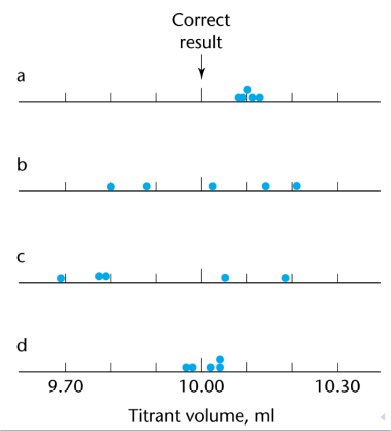
\includegraphics[scale=0.5]{Image10}
\end{center}
\end{frame}

%------------------------------------------------------------------------%

%---------------------------------------------%
\begin{frame}
\frametitle{Accuracy and Precision}
%\frametitle{Method Comparison Studies with \texttt{R}}
\large
\begin{itemize}
\item 
The FDA define precision as the closeness of agreement (degree of
scatter) between a series of measurements obtained from multiple
sampling of the same homogeneous sample under prescribed
conditions. \item Barnhart et al [7] describes precision as being further
subdivided as
\begin{enumerate}
\item  within-run, intra-batch precision or
repeatability (which assesses precision during a single analytical
run), 
\item between-run, inter-batch precision or repeatability
(which measures precision over time)
\end{enumerate} 
\end{itemize}
\end{frame}
%---------------------------------------------%
\begin{frame}
\frametitle{Inter-Method Bias}
\large
\vspace{-1cm}
\begin{itemize}
\item 
In the context of the agreement of two methods, there is also a
tendency of one measurement method to consistently give results
above or below the other method. \item Lack of agreement is a
consequence of the existence of `inter-method bias'. 
\item For two
methods to be considered in good agreement, the inter-method bias
should be in the region of zero. 
\end{itemize}
\end{frame}
\begin{frame}{\bf \tcb{Three Conditions}}
For two methods of measurement to be considered interchangeable, the following conditions must apply (Roy 2009):
\\
\begin{itemize}\itemsep0.5cm
\item No significant inter-method bias
\item No difference in the between-subject variabilities of the two methods
\item No difference in the within-subject variabilities of the two methods (repeatability)
\end{itemize}
\end{frame}

%---------------------------------------------%
\subsection{Grubbs Example}
%---------------------------------------------%
\begin{frame}
\large
\vspace{-1cm}
\begin{itemize}
\item To illustrate the characteristics of a typical method comparison
study consider the data in Table I  (Grubbs 1973). 
\item 


In each of
twelve experimental trials a single round of ammunition was fired
from a 155mm gun, and its velocity was measured simultaneously
(and independently) by three chronographs devices, identified here
by the labels `\textbf{\textit{Fotobalk}}', `\textbf{\textit{Counter}}' and `\textbf{\textit{Terma}}'.
\end{itemize}
\end{frame}






%---------------------------------------------%
\begin{frame}
\large

\begin{table}[ht]
\begin{center}
\begin{tabular}{rrrr}
  \hline
  Round& Fotobalk [F] & Counter [C]& Terma [T]\\
  \hline
  1 & 793.8 & 794.6 & 793.2 \\
  2 & 793.1 & 793.9 & 793.3 \\
  3 & 792.4 & 793.2 & 792.6 \\
  4 & 794.0 & 794.0 & 793.8 \\
  5 & 791.4 & 792.2 & 791.6 \\
  6 & 792.4 & 793.1 & 791.6 \\
  7 & 791.7 & 792.4 & 791.6 \\
  8 & 792.3 & 792.8 & 792.4 \\
  9 & 789.6 & 790.2 & 788.5 \\
  10 & 794.4 & 795.0 & 794.7 \\
  11 & 790.9 & 791.6 & 791.3 \\
  12 & 793.5 & 793.8 & 793.5 \\
   \hline
\end{tabular}
\caption{Velocity measurement from the three chronographs (Grubbs
1973).}
\end{center}
\end{table}
\end{frame}
%---------------------------------------------%
\begin{frame}
\large
\begin{itemize}
\item An important aspect of the these data is that all three methods of
measurement are assumed to have an attended \textbf{\textit{measurement error}}, and
the velocities reported in Table 1.1 can not be assumed to be
`true values' in any absolute sense.
\end{itemize}


%While lack of
%agreement between two methods is inevitable, the question , as
%posed by \alert{BA83}, is 'do the two methods of measurement agree
%sufficiently closely?'
\end{frame}
%---------------------------------------------%
\begin{frame}
\frametitle{Inter-Method Bias}
\large
\begin{itemize}
\item 
A simple estimation of the
inter-method bias can be calculated using the differences of the
paired measurements. \item The data in Table 1.2 (\textit{next slide}) are a good example of
possible inter-method bias; the `Fotobalk' consistently recording
smaller velocities than the `Counter' method.
\item Consequently one
would conclude that there is lack of agreement between the two
methods.
\end{itemize}
\end{frame}
%---------------------------------------------%
\begin{frame}
\large
% latex table generated in R 2.6.0 by xtable 1.5-5 package
% Wed Aug 26 15:22:41 2009
\begin{table}[h!]

\begin{center}

\begin{tabular}{rrrr}
  \hline
 Round& Fotobalk (F) & Counter (C) & F-C \\
  \hline
1 & 793.8& 794.6 & -0.8 \\
  2 & 793.1 & 793.9 & -0.8 \\
  3 & 792.4 & 793.2 & -0.8 \\
  4 & 794.0 & 794.0 & 0.0 \\
  5 & 791.4 & 792.2 & -0.8 \\
  6 & 792.4 & 793.1 & -0.7 \\
  7 & 791.7 & 792.4 & -0.7 \\
  8 & 792.3 & 792.8 & -0.5 \\
  9 & 789.6 & 790.2 & -0.6 \\
  10 & 794.4 & 795.0 & -0.6 \\
  11 & 790.9 & 791.6 & -0.7 \\
  12 & 793.5 & 793.8 & -0.3 \\
   \hline
\end{tabular}
\caption{Difference between Fotobalk and Counter measurements.}
\end{center}
\end{table}
\end{frame}
\end{document}